\documentclass[useAMS,usenatbib]{mn2e}
%\documentclass[twocolumn]{emulateapj}
\usepackage{graphicx,natbib,color,multirow,amsmath}
\voffset=-0.8in

\definecolor{titlecol}{rgb}{0,0,1}
\definecolor{titlecol2}{rgb}{0,0.65,0}
\definecolor{titlecol3}{rgb}{0.99,0.4,0.}

%\definecolor{titledark}{rgb}{0,0,0.8}
%\definecolor{hilit}{rgb}{0,0,1}
%\definecolor{hilitdark}{rgb}{0,0,0.8}
%\font\sbf=cmssbx10 at 32.28pt %big font for headers

\font\nbf=cmssbx10 at 12.28pt %big font for headers

%%%%%%%%%%%%%%%%%%%%%%%%%%%%%%%
%%%% If you want to leave notes in the text feel free to define
%%%% your own colour above and a style below
%%%%%%%%%%%%%%%%%%%%%%%%%%%%%%%
\def\note		{\color{titlecol2} \nbf}
\def\noteb		{\color{titlecol} \nbf}
\def\notebsm	{\color{titlecol}}
\def\notec		{\color{titlecol2} \nbf}
\def\notek		{\color{titlecol3} }

%%%%%%%%%%%%%%%%%%%%%%%%%%%%%%%
% For the eventual referee response
\def\changed    {\color{titlecol} }
%\def\changed    {}


%%%%%%%%%%%%%%%%%%%%%%%%%%%%%%%
%  Other stuff I use a lot
\def\oiii		{$\mathrm{\left[ O \textsc{iii}\right] }$}
\def\moiii		{\mathrm{\left[ O \textsc{iii}\right] }}
\def\nii		{$\mathrm{\left[ N \textsc{ii}\right] }$}
\def\mnii		{\mathrm{\left[ N \textsc{ii}\right] }}
\def\sii		{$\mathrm{\left[ S \textsc{ii}\right] }$}
\def\msii		{\mathrm{\left[ S \textsc{ii}\right] }}
\def\galfit     {{\tt GALFIT}}

\def\mmsun	{\rm{M}_{\odot}}
\def\fnobulge    {$f_{\rm no~bulge}$}
\def\mfnobulge {f_{\rm no~bulge}}
\def\fedgeon     {$f_{\rm edge-on}$}
\def\mfedgeon  {f_{\rm edge-on}}
\def\fcnobulge    {$f_{\rm confirmed~no~bulge}$}
\def\mfcnobulge {f_{\rm confirmed~no~bulge}}


%\def\lesssim{\mathrel{\hbox{\rlap{\hbox{\lower5pt\hbox{$\sim$}}}\hbox{$<$}}}}
%\def\gtrsim{\mathrel{\hbox{\rlap{\hbox{\lower5pt\hbox{$\sim$}}}\hbox{$>$}}}}
%new defs of lesssim gtrsim that I think look better
\def\lesssim{\mathrel{\hbox{\rlap{\hbox{\lower3pt\hbox{$\sim$}}}\hbox{\raise2pt\hbox{$<$}}}}}
\def\gtrsim{\mathrel{\hbox{\rlap{\hbox{\lower3pt\hbox{$\sim$}}}\hbox{\raise2pt\hbox{$>$}}}}}


\newcommand\nodata{ ~$\cdots$~ }




\begin{document}

\title[Galaxy Zoo-CANDELS : Bar Fractions from $0.5 < z < 2$]{Galaxy Zoo-CANDELS : Bar Fractions from $0.5 < z < 2$\thanks{This publication has been made possible by the participation of more than 200,000 volunteers in the Galaxy Zoo project. Their contributions are
individually acknowledged at http://authors.galaxyzoo.org/ .} } 

\author[Simmons et al.]{\parbox[t]{16cm}{{\notebsm Brooke D. Simmons$^{1}\thanks{E-mail: brooke.simmons@astro.ox.ac.uk}$}, 
%% Melvin did analysis & wrote introduction & provided comments & discussion
Thomas Melvin$^{2}$, 
%% Lintott & Masters provided substantial input & comments + many discussions
%% The order of these two is really difficult but Masters also did bar classifications.
Karen Masters$^{2,3}$, 
Chris Lintott$^{1}$, 
%% Note Masters, Melvin, Willett, Keel, Rutkowski, Schawinski, Smethurst, Cheung all provided bar classifications
%% Schawinski's were tragically lost during a bugged-code incident, but they were submitted nonetheless.
%% Also Masters, Melvin, Willett, Keel, Schawinski, Smethurst, Cheung have all given comments on drafts.
%% This sub-list is not in any particular order at the moment.
{\notek Kyle W. Willett$^{X}$}, 
William C. Keel$^{X}$, 
Rebecca Smethurst$^{1}$, 
Edmond Cheung$^{X}$, 
Kevin Schawinski$^{X}$, 
Michael Rutkowski$^{X}$,
%% Have had discussions with Bob that were really helpful as well as written comments - doesn't seem right he's this low but 
%% I think the 8 who submitted 876 classifications apiece should be high too. 
Robert C. Nichol$^{X}$, 
%% Conselice, Mortlock, Hartley, Almaini are citations for inclusion of unpublished UDS specz and photoz data
Christopher Conselice$^{X}$,
Alice Mortlock$^{X}$, 
William Hartley$^{X}$,
Omar Almaini $^{X}$,
Kevin R. V. Casteels$^{X}$, 
Lucy Fortson$^{X}$, 
%% CANDELS is not automatically below GZ but I haven't actually had any comments from anyone on that team yet
[CANDELS - need names], 
names/order still in flux
\vspace{0.1in} }\\
$^{1}$Oxford Astrophysics, Denys Wilkinson Building, Keble Road, Oxford OX1 3RH, UK\\
$^{2}$Institute of Cosmology \& Gravitation, University of Portsmouth, Dennis Sciama Building, Portsmouth PO1 3FX, UK\\
$^{3}$SEPnet,\thanks{www.sepnet.ac.uk} South East Physics Network, School of Physics \& Astronomy, University of Southampton, High�eld, Southampton SO17 1BJ, UK\\
% All or most of these will be needed later
%$^{2}$Yale Center for Astronomy and Astrophysics, Yale University, P.O. Box 208121, New Haven, CT 06520, USA\\
%$^{3}$Department of Astronomy, Yale University, New Haven, CT 06511, USA\\
%$^{4}$Adler Planetarium, 1300 S. Lake Shore Drive, Chicago, IL 60605, USA\\
%$^{5}$Department of Physics, Yale University, New Haven, CT 06511, USA\\
%$^{6}$Astronomy Department, Wesleyan University, Middletown, CT 06459, USA\\
%$^{7}$Blackett Laboratory, Imperial College London, London SW7 2AZ, UK\\
%$^{10}$School of Physics and Astronomy, University of Minnesota, 116 Church St. SE, Minneapolis, MN 55455, USA\\
%$^{11}$Centre for Astronomy and Particle Theory, The University of Nottingham, University Park, Nottingham NG7 2RD, UK
   }
  
\maketitle
  
\label{firstpage}
  
\begin{abstract}

The formation of bars in disks is a tracer of the dynamical maturity of disk galaxy populations. Previous studies have found that the incidence of bars in disks decreases from the local Universe to $z \sim 1$; at $z > 1$, simulations predict that bar features in dynamically mature disks should be extremely rare. 
Here we report the discovery of strongly barred structures in massive disk galaxies at $z \sim 1.5$ in deep rest-frame optical images from CANDELS. From within a sample of 876 disk galaxies identified by visual classification in Galaxy Zoo, we identify 123 barred galaxies (a fraction $f_{bar} = 14.0 \pm 1.5\%$). Selecting
a sub-sample within the same region (brighter than $ L^*$) of the evolving galaxy luminosity function, 
%a volume-limited sub-sample 
we find that the bar fraction does not significantly evolve across the redshift range $0.5 \leq z \leq 2$. We discuss the implications of this discovery in the context of existing simulations and our current understanding of the way disk galaxies have evolved over the last 11 billion years.


  \end{abstract}
  
  \begin{keywords}
  
  galaxies: bars 
  --- 
  galaxies: evolution
  --- 
  galaxies: general 
  --- 
  galaxies: spiral 
  
  \end{keywords}

%%%%%%%%%%%%%%%%%%%%%%%%%%%%%%%%%%%%%%%%%%%%%%
%
%  
\section{Introduction}
%
%
%%%%%%%%%%%%%%%%%%%%%%%%%%%%%%%%%%%%%%%%%%%%%%



Large-scale galactic stellar bars form within dynamically cold, rotationally supported disks \citep{athanassoula05b, combes09, sellwood10,athanassoula13}. Thus the evolution of the fraction of disk galaxies with bar features traces the overall evolution of disk galaxy dynamics. Locally, bars are present in $\sim 25 - 50\%$ of disk galaxies \citep[e.g.][]{odewahn96a, d_elmegreen04b, aguerri09, nair10, masters11a, cheung13}, with their abundance steadily decreasing to $\sim$10\% of disk galaxies at $z \sim 1$ \citep{abraham99, d_elmegreen04b, d_elmegreen05, sheth08, melvin14}. 

The lower incidence of bars at higher redshifts may be in part be due to the increased incidence of mergers and galaxy interactions \citep{conselice03b, lotz11, casteels13}, which disrupt and heat disks, destroying or preventing the formation of bars. It may also be related to the expected increase in disk gas fraction with redshift; this has been observed indirectly via the increase in specific star formation rate to $z \sim 2$ \citep[e.g.,][]{lilly96,madau98}, and directly via the increased $M_{gas}/M_{star}$ from CO observations (e.g., \citeauthor{tacconi10} \citeyear{tacconi10}, \citeyear{tacconi13}; for a detailed review, see \citeauthor{carilli13} \citeyear{carilli13}). Bars in galaxies are observed to be anti-correlated with specific star formation rate \citep{cheung13} and disk gas fraction \citep{masters12a} in agreement with theoretical predictions \citep[][though a high gas fraction does not entirely preclude the existence of a bar; \citeauthor{nair10} \citeyear{nair10}; \citeauthor{masters12a} \citeyear{masters12a}]{friedli93, berentzen07, villavargas10, athanassoula13}. 

The current theoretical understanding of bar fraction evolution suggests that disk galaxies at $z > 1$ are too dynamically hot to form bars (e.g., \citeauthor*{kraljic12} \citeyear{kraljic12} find no observable bars within a simulated sample of galaxies at $z \sim 1.5$). Other simulations explore the impact of tidal heating and galaxy harassment, which can either inhibit bar formation \emph{or} promote it, depending on mass \citep[with higher-mass galaxies being more likely to form a long-lasting bar due to a minor merger or interaction;][]{noguchi88, moore96, skibba12}. Testing this requires high-resolution imaging over large areas to observe statistically significant samples with sufficient $\Delta z$ resolution to observe evolution and adequate spatial resolution to resolve galactic-scale bars in the rest-frame optical \citep[since the detectability of bars decreases rapidly blueward of the 4000 \AA\ break;][]{sheth08}.

These observing requirements currently limit studies of disk populations via bar fractions to surveys with the \emph{Hubble Space Telescope (HST)}. Previous studies have used the optical cameras on \emph{HST} to examine bar fractions to $z \sim 1$. 
% Lucy suggests I cite Chris' original paper to have some bibliographical parity with CANDELS but I can't quite see how to do that without making it seem as though we're using classifications from 2008. There might be a way of saying explicitly that these are first results from Galaxy Zoo-CANDELS and that an overview of Galaxy Zoo is at Lintott et al. without it seeming too obvious...
In this paper, we use Galaxy Zoo morphological classifications of galaxies imaged by the Cosmic Assembly Near-Infrared Deep Extragalactic Legacy Survey \citep[CANDELS;][]{grogin11,koekemoer11}, which uses \emph{HST's} near-infrared Wide-Field Camera 3 (WFC3) to extend the redshift range within which high-resolution rest-frame optical galaxy images are available to $z \gtrsim 2$.

In Section 2 we describe our sample selection, including a summary of Galaxy Zoo classifications of CANDELS galaxies and how disks and bars are selected. We also explore any potential biases that may affect our results. We present our results in Section 3, with a discussion including comparison to simulated predictions in Section 4, and a summary in Section 5. Throughout
this paper we use the AB magnitude system, and where necessary we adopt a cosmology consistent with $\Lambda$CDM, with $H_{\rm 0}=70 {\rm
km~s^{-1}}$Mpc$^{\rm -1}$, $\Omega_{\rm m}=0.3$ and $\Omega_{\rm \Lambda}=0.7$ \citep{bennett13}.




%%%%%%%%%%%%%%%%%%%%%%%%%%%%%%%%%%%%%%%%%%%%%%
%
%
\section{Data}\label{sec:data}
%
%
%%%%%%%%%%%%%%%%%%%%%%%%%%%%%%%%%%%%%%%%%%%%%%

\subsection{CANDELS}\label{candelsdata}

The Cosmic Assembly Near-infrared Extragalactic Legacy Survey \citep[CANDELS;][]{grogin11} is an \emph{HST} Treasury program combining optical and near-infrared imaging from the Advanced Camera for Surveys (ACS) and Wide Field Camera 3 (infrared channel; WFC3/IR) across five well-studied survey fields 
% Re: a suggestion from LF, I'm not sure it's correct to cite the release papers for these surveys as here I'm only referring to the fields themselves, not the surveys/data that came before -- where I'm using the redshift data below I will certainly cite.
(GOODS-North and -South, EGS, UDS and COSMOS) and at two depths, ``wide'' and ``deep''. The wide fields are imaged at 2--3-orbit depths, and the deep fields at $\sim$13-orbit depths, over multiple epochs. These are reduced and combined \citep[a process described in detail by][]{koekemoer11} to produce a single mosaic for each field, with drizzled resolutions of $0.03^{\prime\prime}$ and $0.06^{\prime\prime}$ per pixel for ACS and WFC3/IR, respectively.

Here we use the CANDELS ACS and WFC3/IR images from within the COSMOS, GOODS-South, and UDS fields for which raw classifications from the Galaxy Zoo project are presently available. The WFC3/IR observations of these fields cover approximately 0.3 square degrees combined. The Galaxy Zoo classifications are based on colour images created using an asinh stretch \citep{lupton04} with WFC3 F160W, F125W, and ACS F814W as red, green and blue channels respectively. 
% Triple-check this.
Some of the colour images use ACS data that was observed during previous surveys \citep{giavalisco04,scoville07,notsureonUDS} and re-analysed by the CANDELS pipeline.


\subsection{Classifications}\label{sec:gzdata}

Galaxy Zoo provides quantified visual morphologies by obtaining multiple independent classifications for each galaxy. Beginning in 2007, more than 1,000,000 galaxy images total from both the Sloan Digital Sky Survey and the \emph{HST} have each been classified by typically $\sim 40$ independent volunteers via a web interface\footnote{zoo4.galaxyzoo.org}. The initial version of the project \citep{lintott08,lintott11} asked a single question per galaxy (whether the galaxy was spiral or elliptical). Subsequent versions have collected more detailed morphological information, including finer sub-structures of disk galaxies such as bulge strength and bars, via a tiered classification tree \citep[e.g.,][]{willett13,melvin14}. 

This work uses classifications collected during the fourth release of Galaxy Zoo, specifically of 49,555 images from the COSMOS, GOODS-South, and UDS fields in the CANDELS survey (hereafter GZ-CANDELS). The dataset was composed of all sources having $F160W$ ($H$) apparent magnitude $< 25.5$. Initial analysis after each galaxy had received typically $\sim 20$ classifications resulted in the early retirement of 1,555 point-like sources and 11,837 faint, low-surface brightness galaxies without resolvable fine features. Although the project is still ongoing, 
%{\notek (We've stopped now, no?} {\notebsm Still have EGS and GOODS-N to go, plus simulations + FERENGI-CANDELS)}, 
as of the date of this analysis each of the remaining objects has received at least 40 independent classifications.

The classification tree used for GZ-CANDELS (Simmons et al., in preparation; see Figure \ref{fig:sampleselection} for the portion relevant here) first asks volunteers to choose whether a galaxy is mostly smooth, has features, or is a star/artifact. The bar classification question (``Is there a sign of a bar feature through the centre of the galaxy?'') is reached once a volunteer has chosen ``Features or Disk'' as an answer to the first question and has subsequently said the galaxy does \emph{not} have a mostly clumpy appearance, nor is it an edge-on disk. The bar question is therefore a fourth-tier task, and the number of volunteers per galaxy who answer the bar question varies depending on each volunteer's responses to the earlier tasks. {\notek May want to be careful with vocab: distinguish between tasks, responses, questions, and answers within GZ.} {\notebsm Agreed we should be consistent across papers/GZ releases. Is this not? Feel free to correct it.}




%%%%% [FIGURE: Bar fractions and mags of sample] %%%%%
\begin{figure*}
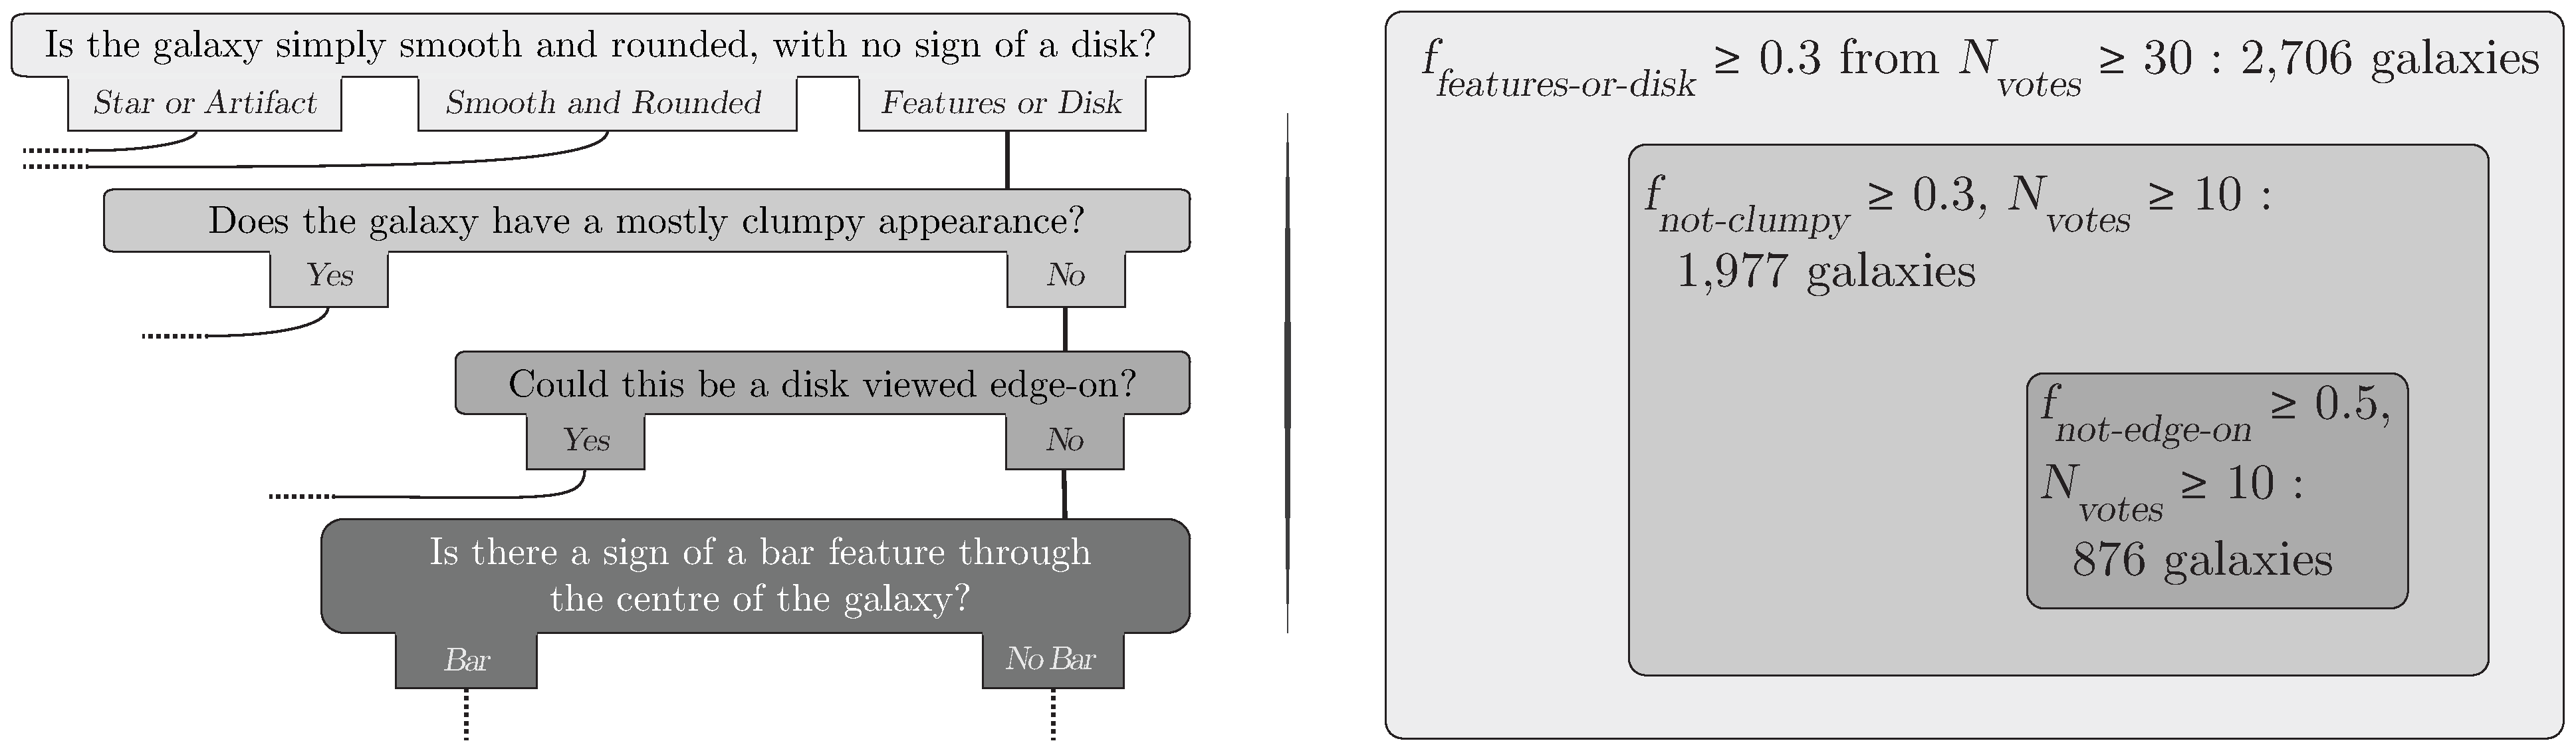
\includegraphics[scale=0.273]{tree_part_with_selection.eps}
\caption{
\emph{Left:} Partial Galaxy Zoo-CANDELS classification tree, starting with the first question (top) and leading to the bar feature question. There are 17 questions total in the tree; the bar question is a 4th-tier task. \emph{Right:} Selection of the featured, not-edge-on disk galaxy sample (876 galaxies) in GZ-CANDELS. This selection was made independently of restrictions on redshift or luminosity (a full description of the sample selection is described in Section \ref{sec:sample}). Eight independent classifiers subsequently examined each of the 876 disk galaxies for evidence of a bar. 
%{\notek Great diagram. Include the final luminosity-limited disk sample?} {\notebsm I figured this was for the morphological selection only, as the redshift and L cuts are a separate step.}
}
\label{fig:sampleselection}
\end{figure*}
%%%%% END FIGURE %%%%%


\subsection{Redshifts}\label{sec:z}

Each of the fields covered by CANDELS data has considerable ancillary data from previous and ongoing work. We assemble photometric and spectroscopic redshifts from the available literature. For galaxies in the COSMOS field, we combine spectroscopic redshifts from the zCOSMOS project \citep{lilly07} with photometric redshifts from COSMOS \citep{ilbert09} and from the NEWFIRM medium-band survey \citep{whitaker11}. In the GOODS-South field, we use the catalog of \citet{cardamone10b}, who added photometric redshifts based on deep broad- and medium-band data from MuSYC \citep{gawiser06} to available spectroscopic redshifts compiled from multiple sources \citep{yes,you,must,cite,them,all,dont,be,lazy}. In the UDS field, we use available spectroscopic \citep{ref1, ref2, ref3} and photometric \citep{mortlock13} redshifts, the latter of which make use of deep multi-wavelength coverage from UKIDSS as well as $J$ and $H$-band magnitudes from CANDELS \citep[similar to photometric redshifts calculated by, e.g.,][]{candelsphotozref}. Of the 49,555 galaxies originally included in Galaxy Zoo-CANDELS, 46,234 currently have spectroscopic (2,886) or photometric (43,348) redshifts.




\subsection{Sample Selection}\label{sec:sample}

%%%%% [FIGURE: Example images] %%%%%
\begin{figure*}
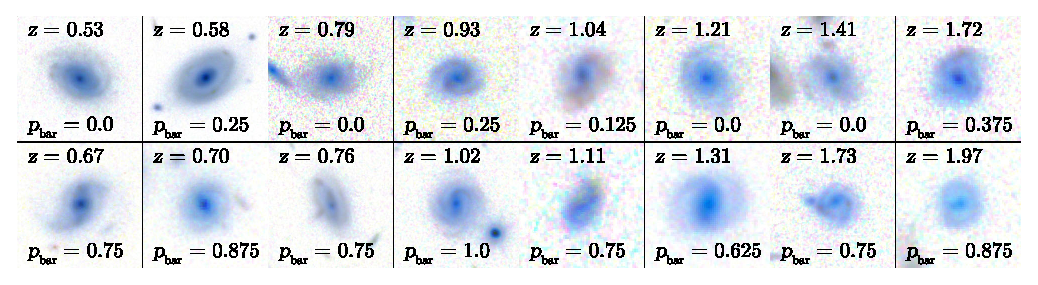
\includegraphics[scale=1.0]{barfig_3.eps}
\caption{
Examples of disk galaxies in GZ-CANDELS whose bar vote percentage $(p_{bar})$ is below (top row) and above (bottom row) the threshold for inclusion in the barred sub-sample. 
}
\label{fig:gals}
\end{figure*}
%%%%% END FIGURE %%%%%


A full reduction of the GZ-CANDELS classifications, resulting in a catalog of morphological votes for each galaxy, is ongoing. Here we use the raw vote percentages, which have been neither weighted nor debiased. The effects of using raw versus the reduced classifications are twofold. First, the unweighted votes are likely biased in the first question toward an excess of votes for ``Star or Artifact'' (see \citeauthor{willett13} \citeyear{willett13} for a discussion of how inconsistent votes are downweighted in Galaxy Zoo 2). Second, the effects of surface brightness dimming and loss of spatial resolution are not accounted for in the vote percentages, which is potentially a significant effect in a sample extending to $z \sim 2$ in the rest-frame optical.

To minimize the impact of the lack of user weighting, we employ a lower vote percentage threshold when selecting ``featured'' galaxies compared to thresholds using weighted data. We select as ``featured'' galaxies those where at least 30\% of votes (out of at least 30 volunteers total) were registered for ``Features or Disk''. This selects 2,706 featured galaxies. After the first question, the user weighting used by previous Galaxy Zoo data reductions affects vote percentages by typically no more than a few percent; we therefore expect the lack of weighting to have little to no systematic effect on additional vote percentages. {\notek I hope that's true, but it really hasn't been shown explicitly. Something for BDS, KW, SB et al. to work on.} {\notebsm I looked at this in some detail when I started playing with GZH results. Once you get past the first question the difference in any given vote percentage between using weighted and unweighted is typically less than $\sim 3$\%.}

Subsequent to the featured galaxy selection, we select a sub-sample where at least 30\% of volunteers (where a minimum of 10 answered the question) registered a vote for ``no'' to the question ``Does the galaxy have a mostly clumpy appearance?'' in order to remove galaxies whose features do not clearly include a disk; this selection removes 729 clumpy galaxies in total. We include this selection in order to consider each branch of the classification tree that leads to the bar-feature question; however, we note that were we to ignore the clump-threshold criterion completely, this would only cause contamination of the final ``featured'' sample at the 1\% level. Our qualitative results are thus not sensitive to the specific choice of clumpy threshold between $0.1 \leq p_{\mathrm not-clumpy} \leq 0.6$.

%%%%% [FIGURE: Volume-limited sample] %%%%%
\begin{figure}
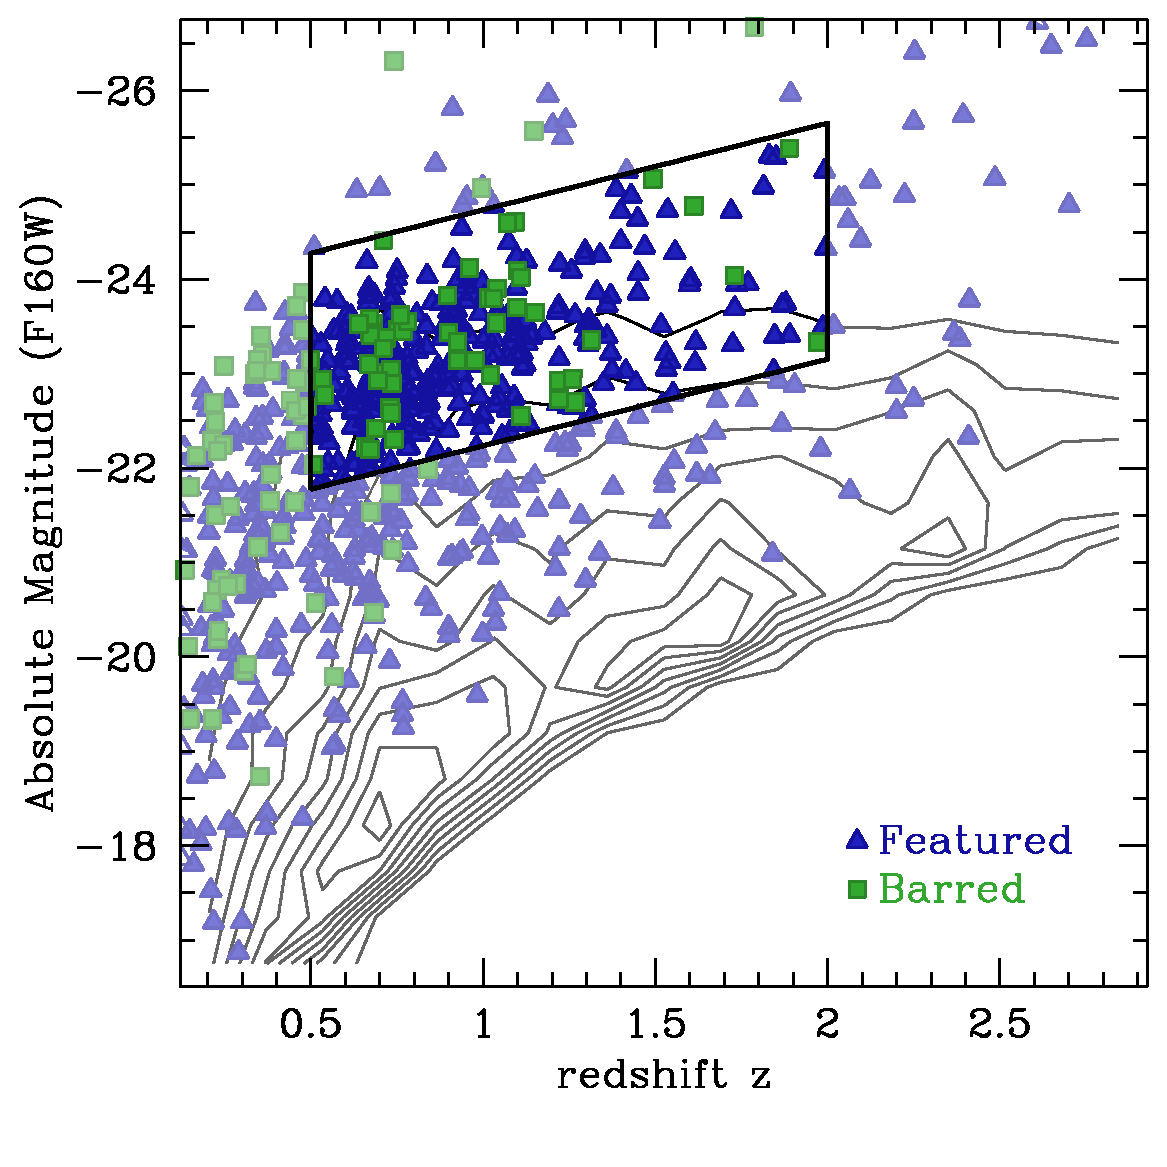
\includegraphics[scale=0.41]{Mag_z_contours.eps}
\caption{
Absolute $H$-band magnitude versus redshift for all sources with $H < 25.5$ (contours in steps of 10\%) and 876 ``Featured'' not-edge-on disks (blue triangles), of which 123 galaxies show clear evidence of a bar (green squares). To facilitate comparison between lookback times, avoid biases due to surface-brightness dimming when calculating bar fractions, and ensure all observed $H$-band flux is redward of the 4000-\AA\ break, we select sub-samples within the same region of the evolving galaxy luminosity function \citep{marchesini12} and $0.5 \leq z \leq 2$ (parallelogram). Within this region there are 370 not-edge-on disk galaxies, 56 of which have clear evidence of bars.
}
\label{fig:mag_z}
\end{figure}
%%%%% END FIGURE %%%%%



Further, we also require that 50\% of volunteers (of at least 10) registered a vote for a disk galaxy that is ``not-edge-on''.
This threshold choice is higher to reflect a more conservative requirement that a bar always be detectable in the sample of disk galaxies (though the thresholds used to select disk features are less strict to slightly favour completeness). This selects a sample of 876 featured disk galaxies from which a bar may be identified, if it exists. Figure \ref{fig:sampleselection} shows a visual representation of this sample selection, from which a further sub-sample of barred galaxies may be identified. However, approximately 20\% of these 876 galaxies received less than 10 raw votes \emph{total} for the question ``Is there any sign of a bar feature through the centre of the galaxy?'', a consequence of the broad initial selection of featured galaxies and the multiply-branched nature of the classification tree. Because of the lower number of votes per galaxy in the 4$^{\rm{th}}$ tier of the classification tree (the position of the bar question), within the featured sample the raw bar fractional vote is statistically useful, but uncertain for individual galaxies.

We therefore elected to supplement the volunteer data with visual classifications from the Galaxy Zoo science team to select the sub-sample of barred disk galaxies. Eight of the authors\footnote{BDS, TM, KWW, WCK, MR, KLM, RS, EC} inspected each of the 876 featured disk galaxies for evidence of a bar; these votes were unanimous approximately 60\% of the time, either for a bar feature (23 galaxies) or no bar (512 galaxies). Among galaxies where the science team voted unanimously that a bar is present, the mean volunteer bar vote percentage is  $0.65 \pm 0.15$. Among galaxies where the science team was unanimous that a bar is \emph{not} present, the mean volunteer bar vote percentage is $0.11 \pm 0.11$. The science team and volunteer bar vote percentages generally correlate, although the low number of volunteer votes for many objects means the dispersion in the correlation is high. Following vote percentage thresholds used in previous studies \citep[this method has been shown to select strong bars;][]{masters11a,willett13,melvin14}, we mark a galaxy as barred if at least half of the science-team classifiers indicated the presence of a bar ($p_{bar} \geq 0.5$). 
%We also note that this vote fraction threshold is statistically identical to a vote threshold of 45\% among volunteer votes (123 barred galaxies from science team votes vs. 121 from raw volunteer votes), but the overlap is only approximately 70\%.
%

The absolute $H$-band magnitudes in the sample are plotted as a function of redshift in Figure \ref{fig:mag_z}. Of the featured not-edge-on (and barred) galaxies, 525 (61) have redshifts between $0.5 \leq z \leq 2.0$. Within this redshift range, all flux collected by the WFC3 $H$ band is redward of the 4000-\AA\ break. Examples of barred and unbarred galaxies are shown in Figure \ref{fig:gals}.

To minimize any bias caused by surface-brightness dimming at higher redshifts, we additionally employ a conservative luminosity cut when examining bar fractions, choosing a minimum $H$ absolute magnitude of $-23.15$ at $z = 2$ (or approximately an apparent $H= 23.5$). This ensures that featured galaxies can be detected within the sub-sample at all $z < 2$. We note that this is brighter than the knee of the rest-frame-$V$-band luminosity function at this redshift \citep{marchesini12}. In order to examine similar populations across our entire redshift range, we use a varying luminosity cut based on selecting the same region of the evolving luminosity function \citep[corrected to observed $H$ band;][]{blanton07,marchesini12}: this selection is shown as a parallelogram shape in Figure \ref{fig:mag_z}. This final cut produces 370 featured, not-edge-on disk galaxies, of which 56 have strong bar signatures. We note that our results are robust to small variations in the redshift and luminosity thresholds chosen for the sample.
% Note the high-L cut also helps avoid issues caused by the significant variations in completeness with magnitude across the various CANDELS fields, and even within individual CANDELS fields (e.g. GOODS-S has ERS, wide and deep). 




%%%%%%%%%%%%%%%%%%%%%%%%%%%%%%%%%%%%%%%%%%%%%%
%
%
\section{Results: Bar fractions}\label{sec:results}
%
%
%%%%%%%%%%%%%%%%%%%%%%%%%%%%%%%%%%%%%%%%%%%%%%

The fraction of disk galaxies with visually identified strong bars between $0.5 \leq z \leq 2$ is $\sim$1$0-20$\%, independent of any reasonable {\notek (def.)} selection on luminosity ranges or vote fractions for detected features, lack of clumpiness, disk inclination angle, and strong bar features. Figure \ref{fig:barfrac} shows the bar fraction with lookback time, from $t_{lb} = 5.0$~Gyr ($z = 0.5$) to 10.2~Gyr ($z=2.0$). The sample encompasses the same subset of the galaxy luminosity function relative to the evolving $L^*$; the conservative selection to ensure detectability of features (or lack thereof) to $z = 2$ means the galaxies examined here are all brighter than $L^*$ at their epoch. 

Within this sample, and given the uncertainties, the bar fraction is consistent with zero evolution between $1 < z < 2$. Many studies of the bar fraction at $z \lesssim 1$ find that the bar fraction does evolve, though these findings are not unanimous \citep{abraham96,abraham99,jogee04,d_elmegreen04b,d_elmegreen05,sheth08,cameron10,melvin14}. Although the details depend on both the bar selection method being used and the properties of the galaxies themselves, disk galaxies are generally more likely to show strong bar features at lower redshift. Two independent studies of the full COSMOS-ACS sample \citep{sheth08,melvin14} show that the fraction of visually identified strong bars decreases with redshift, from approximately 35\% at $z = 0.2$ to 15\% at $z = 1$. 

%%%%% [FIGURE: Bar fractions and mags of sample] %%%%%
\begin{figure}
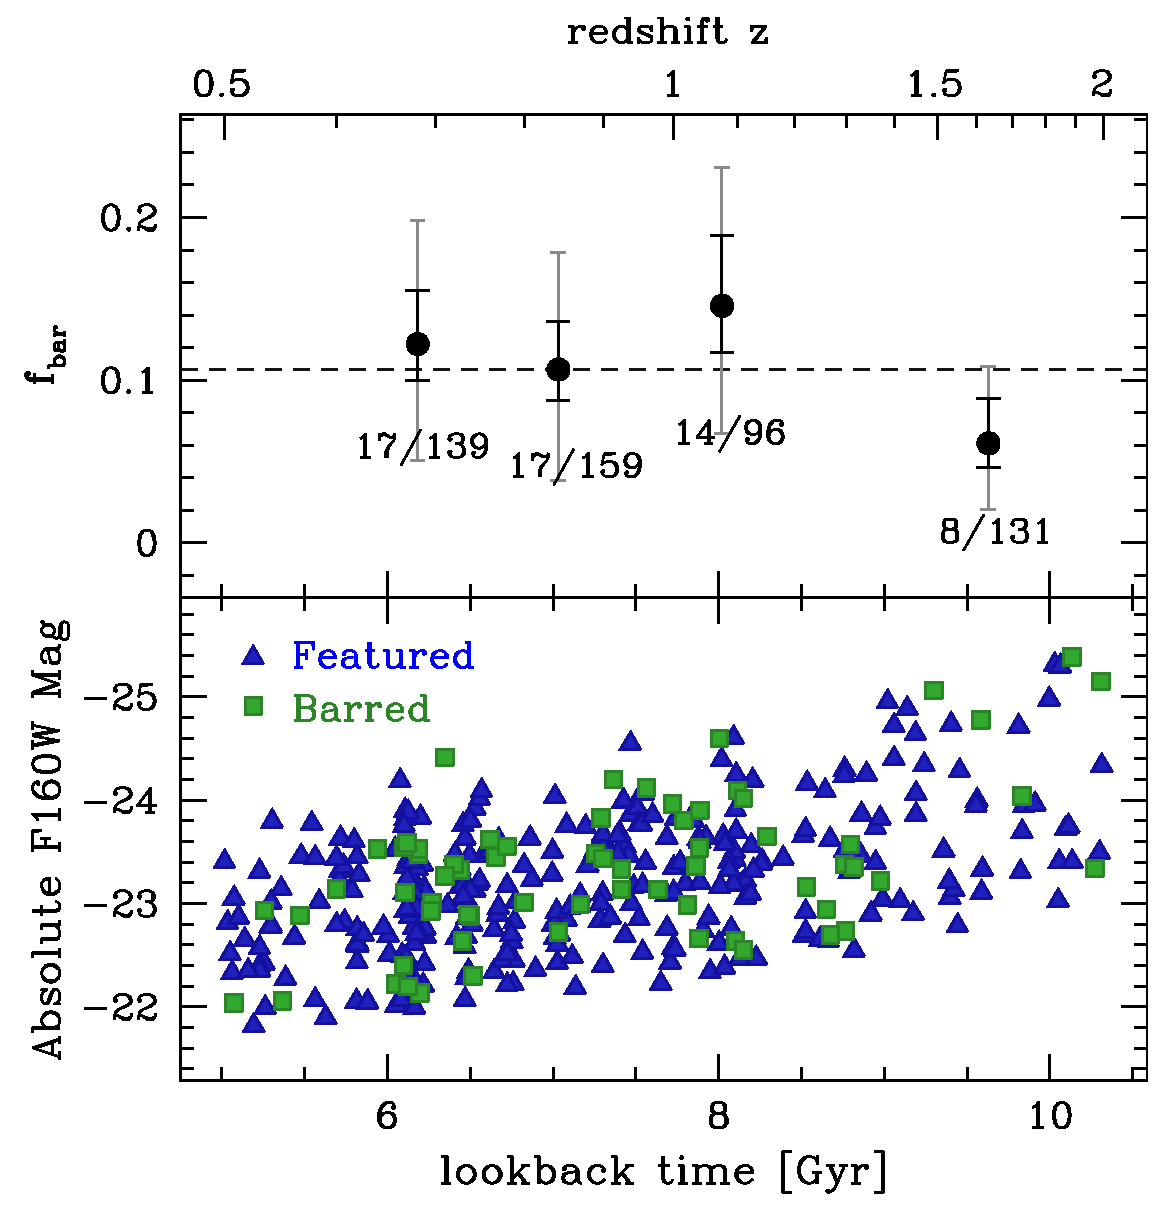
\includegraphics[scale=0.425]{barfrac_Mag_t.eps}
\caption{
\emph{Top panel:} Bar fraction versus lookback time. Uncertainties are binomial error bars \citep{gehrels86}; within these uncertainties, the bar fraction is consistent with no evolution from $0.5 \leq z \leq 2$. Bins were chosen to enclose similar lookback time intervals; the bar fraction across all bins ($15 \pm 2$\%) is shown as a dashed line. \emph{Bottom panel:} absolute $H$-band magnitudes of the sample from which the fractions are drawn.
}
\label{fig:barfrac}
\end{figure}
%%%%% END FIGURE %%%%%


%%%%% [FIGURE: These results in context] %%%%%
\begin{figure}
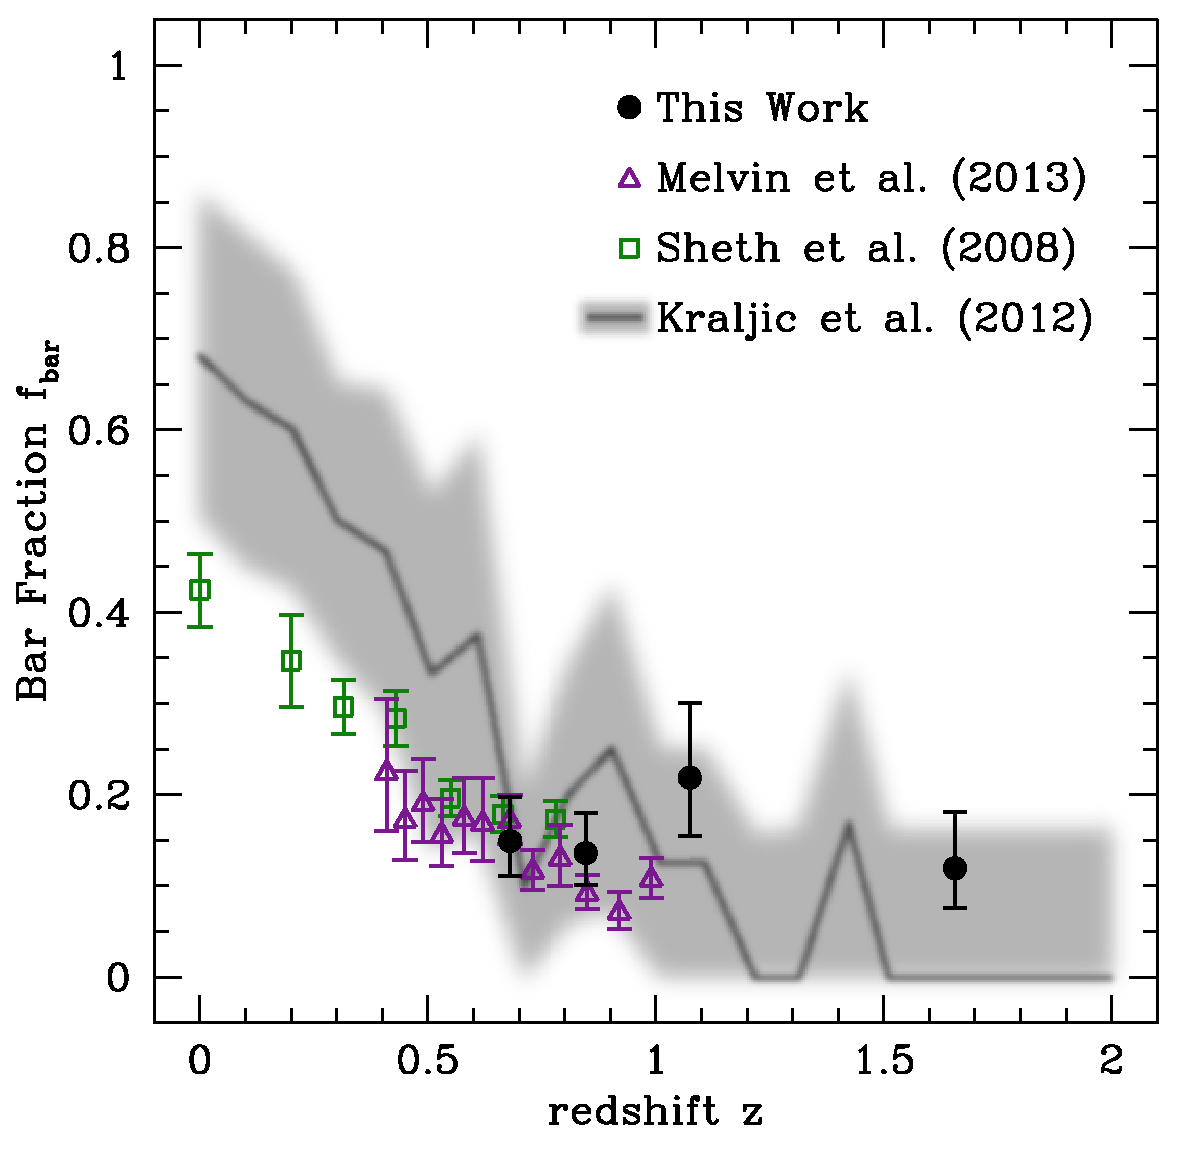
\includegraphics[scale=0.425]{barz_axes_withsims_strongbars.eps}
\caption{
Fraction of disk galaxies having a strong bar feature versus redshift, in the context of other work assessing visual strong bar fraction. 
Uncertainties in observed and predicted fractions were calculated assuming binomial statistics \citep{gehrels86}; 
the $1 \sigma$ error bars for the \citet[][Ma11, blue cross]{masters11a} and \citet[][dV91, red diamond]{RC3} fractions are smaller than the size of the points and are omitted.
At higher redshift, bar fractions in this work (black circles) at $z < 1$ are consistent with those of \citet[][S08, green squares]{sheth08}  and \citet[][Me14, purple triangles]{melvin14} despite differences in selection methods. 
\citet[][K12]{kraljic12} computed the fraction of strong bars to $z=2$ among disk galaxies that evolved to stellar masses $M_\ast \approx 10^{10-11} \mmsun $ (shaded region); the predicted bar fraction is consistent with that observed here within the uncertainties, although we note that differences between simulated and observed mass/luminosity ranges make direct quantitative comparisons more difficult.
}
\label{fig:barfrac_context}
\end{figure}
%%%%% END FIGURE %%%%%


Figure \ref{fig:barfrac_context} shows the visually identified strong bar fraction versus redshift in the context of other work, both observational and theoretical. Within the redshift range where we overlap with other observational studies, the bar fraction is consistent. However, the bar fraction evolution appears to cease at $z > 1$; our result is not consistent with a simple extrapolation of the decreasing bar fraction trend found by other studies. 

Using zoom-in cosmological simulations of 33 field and loose group galaxies, \citet{kraljic12} find that disk galaxies at $z \gtrsim 1$ 
% KLM comment: should this be "the progenitors of z ~ 0 disk galaxies, observed at z > 1"? BDS answer: in this case the plot shows the progenitors that are also disks at z > 1. But yes, all are progenitors of disk galaxies -- it's just not the full Kraljic sample.
are generally too dynamically hot to become unstable to bar formation; this manifests itself as a decreasing bar fraction with increasing redshift. Although the quantitative bar fractions in their simulations depend on the threshold used to define a bar feature, the fraction of disk galaxies hosting bars drops to zero, or near zero, by any definition they use \citep[Figure \ref{fig:barfrac_context} shows their standard ``strong bar'' definition, which is the closest to observational samples defined by visual classifications such as those here and in previous work;][]{masters11a,willett13,melvin14}. This initially appears inconsistent with our results showing a low, but non-zero, bar fraction. However,  due to the small simulated sample size of \citeauthor{kraljic12} compared to observational studies, a complete lack of bar feature detection within the subset of their sample identified as disk galaxies is consistent with a bar fraction of $\approx 15$\% within uncertainties. 

We also note that the galaxy masses and luminosities used in the simulations were on average lower {\notek (How much?)} than those examined in this work, making a direct comparison to this work more difficult, as bar fraction also depends on stellar mass \citep{sheth08,melvin14}. \citeauthor{kraljic12} predict that massive disk galaxies will be more likely to form bars at higher redshift than lower mass disk galaxies due to higher-mass galaxies reaching dynamical maturity at earlier epochs. This is qualitatively consistent with our finding that the bar fraction at $z \sim 2$ is approximately $10-20$\% within $1 \sigma$ binomial uncertainties, but a direct and quantitative theoretical comparison to our observational result is currently not possible given available simulations. New simulations encompassing galaxies with higher stellar masses would help to advance this field further.

Our results agree with previous work that the epoch of bar formation in the disk galaxy population begins at $z < 1$. However, bars are not completely absent even at $z \sim 2$: some disks at the masses probed by our sample are mature enough even by this epoch ($\sim 3-4$ Gyr after the Big Bang) to host a bar. 

Whether the bar features are analogous to long-lived bars in dynamically cold disks at lower redshift or are shorter-lived features triggered within dynamically warmer disks is unclear from examination of bar fractions alone. Examination of individual simulated galaxies by \citeauthor{kraljic12} indicates that bars formed at $z > 1.5$ tend to undergo shorter cycles of formation and destruction., and there is some evidence that short-lived grand design spiral features more commonly associated with mature disks can be triggered by interactions at $z > 2$ \citep{law12}. 

Thus the incidence of bars in massive high-redshift disks may be due at least in part to galaxy interactions and mergers, combined with shorter bar lifetimes due to dynamically warmer disks. Minor galaxy mergers may dynamically heat a disk and destroy a bar, or they may trigger the formation of a bar, depending on the particulars of the interaction \citep{gerin90,berentzen03,berentzen04}. The relative likelihood of these contrasting end results, combined with the incidence of minor mergers among this population at $z \sim 2$, may combine to produce a net effect that stabilizes the bar fraction at $z \sim 10$\% during this epoch of galaxy assembly. 

{\notek That's intriguing. Can the GZ results say anything about the fraction of disks that look dynamically disturbed, either from volunteer data or re-examination by us? Maybe we could look at how $f_{odd}$ or $f_{merger}$ differs among barred and non-barred galaxies?} {\notebsm There's no longer an $f_{odd}$, but we do have the merger fraction and $f_{tidal}$; at least a first look is within scope and definitely a good idea.}






%%%%%%%%%%%%%%%%%%%%%%%%%%%%%%%%%%%%%%%%%%%%%%
%
%  
\section{Summary}
%
%
%%%%%%%%%%%%%%%%%%%%%%%%%%%%%%%%%%%%%%%%%%%%%%

Using visual classifications of rest-frame optical \emph{HST} galaxy images from the ongoing Galaxy Zoo-CANDELS project, we examined for the first time the fraction of disk galaxies hosting a bar feature to $z \sim 2$ in order to trace the dynamical state of disks as early as $\sim 3$~Gyr after the Big Bang. We find that the bar fraction to $z \sim 1$ is consistent with previous studies using similar analysis methods. 

At $z > 1$, the bar fraction is approximately $10-20$\% and consistent with no evolution between $1 < z < 2$. This is qualitatively consistent with the predictions of zoom-in cosmological simulations, although further work is needed to determine whether simulations of disk galaxies with $L > L^*$ predict the same quantitative strong bar fraction at $z < 2$. 

That the bar fraction from $1 < z < 2$ appears to be small but constant among massive disk galaxies implies that massive disk dynamics do not rapidly change on average over this period. Further clarification may come in the future when additional detailed morphological classifications of deep $z \sim 2$ rest-frame optical galaxy images are available; future comparison with independent morphologies of the same galaxies  \citep{kartaltepe14} as well as additional simulations will help provide a more nuanced understanding of the underlying physical causes of this apparently stable bar fraction. 
  
%%%%%%%%%%%%%%%%%%%%%%%%%%%%%%%%%%%%%%%%%%%%%%
%
%
\section*{Acknowledgments}
%
%
%%%%%%%%%%%%%%%%%%%%%%%%%%%%%%%%%%%%%%%%%%%%%%

%The authors wish to thank to C. Peng for making \galfit\ publicly available, and for many enlightening discussions.  We also wish to thank R. Skibba, M. Williams, and the anonymous referee for thorough and constructive comments that helped us improve this manuscript.
%
TOPCAT \citep{taylor05} and an OS X widget form of the JavaScript Cosmology Calculator \citep{wright06} were used while preparing this paper. 
%
BDS gratefully acknowledges support from the Oxford Martin School, Worcester College and Balliol College, Oxford.
%
KS gratefully acknowledges support from Swiss National Science Foundation Grant PP00P2\_138979/1. 
%
TM acknowledges funding from the Science and Technology Facilities Council ST/J500665/1.
%
\textbf{Please send your grant acknowledgments at your earliest convenience.}
%
% Old acknowledgments:
%Support for the work of KS was provided by NASA through Einstein Postdoctoral Fellowship grant number PF9-00069, issued by the Chandra X-ray Observatory Center, which is operated by the Smithsonian Astrophysical Observatory for and on behalf of NASA under contract NAS8-03060.
%
%ECM acknowledges support from the National Science Foundation through grant AST-0909063.
%
%SK acknowledges fellowships from the 1851 Royal Commission, Imperial College London, Worcester College, Oxford and support from the BIPAC institute at Oxford.
%
%KLM acknowledges funding from The Leverhulme Trust as a 2010 Early Career Fellow.
%
%SPB acknowledges receipt of an STFC Advanced Fellowship.
%
%RCN acknowledges STFC Rolling Grant ST/I001204/1 to ICG for �Survey Cosmology and Astrophysics�. 

The development of Galaxy Zoo was supported in part by the Alfred P. Sloan Foundation. Galaxy Zoo was supported by The Leverhulme Trust. 

{\noteb CANDELS ACKNOWLEDGMENT} {\notebsm -- BDS to look this up}

%This publication makes use of data products from the Wide-field Infrared Survey Explorer, which is a joint project of the University of California, Los Angeles, and the Jet Propulsion Laboratory/California Institute of Technology, funded by the National Aeronautics and Space Administration.

%Funding for the SDSS and SDSS-II has been provided by the Alfred P. Sloan Foundation, the Participating Institutions, the National Science Foundation, the U.S. Department of Energy, the National Aeronautics and Space Administration, the Japanese Monbukagakusho, the Max Planck Society, and the Higher Education Funding Council for England. The SDSS Web Site is http://www.sdss.org/.

%The SDSS is managed by the Astrophysical Research Consortium for the Participating Institutions. The Participating Institutions are the American Museum of Natural History, Astrophysical Institute Potsdam, University of Basel, University of Cambridge, Case Western Reserve University, University of Chicago, Drexel University, Fermilab, the Institute for Advanced Study, the Japan Participation Group, Johns Hopkins University, the Joint Institute for Nuclear Astrophysics, the Kavli Institute for Particle Astrophysics and Cosmology, the Korean Scientist Group, the Chinese Academy of Sciences (LAMOST), Los Alamos National Laboratory, the Max-Planck-Institute for Astronomy (MPIA), the Max-Planck-Institute for Astrophysics (MPA), New Mexico State University, Ohio State University, University of Pittsburgh, University of Portsmouth, Princeton University, the United States Naval Observatory, Yale University and the University of Washington. 
  
\bibliographystyle{mn2e}
\bibliography{refs}  

\appendix
\section{Possible sources of error in bar fractions}

There are several potential sources of error that could affect our results. Below we address these and discuss their potential impact on the results presented here. 

\begin{itemize}
\item \emph{Missing disk galaxies:} 
as disks with an exponential light profile fall below the noise limit more quickly as a function of redshift than more concentrated bulges, it is possible that a study could preferentially miss disks at high redshift. The bar fraction could be affected if volunteers preferentially identified bars (which can have higher surface brightnesses than the outer parts of disks) as ``featured'', but equally a galaxy where only the bar was visible might be classified as edge-on and thus be excluded from a disk galaxy sample such as that used here. 

In general, surface brightness limits are a significant concern in any study of bar fractions. This motivated the conservative lower luminosity limit (Section \ref{sec:sample}). Additionally, we have chosen to sample the same part of the galaxy luminosity function (relative to the evolving ``knee'') across our redshift range. This minimizes the loss of disk galaxies in the lower-redshift part of the sample versus a luminosity-limited approach that samples brighter, rarer galaxies compared to the bulk of the population as the sample redshift decreases. For both of these reasons as well as the depth of the CANDELS images, it is likely that the underlying sample selection does not bias against detection of disk galaxies.

Additionally, our relatively broad selection of galaxies with ``Features or Disk'' within Galaxy Zoo is designed to account for the systematic downward shift of unweighted vote fractions that have not been corrected for (in particular) errant ``Star or Artifact'' selections. Accounting for this in the first morphological selection prevents it from systematically affecting the rest of the classifications, as errant selections are removed from the rest of the classification tree so do not affect further branches. We also note that the bar fraction results discussed in Section \ref{sec:results} are not strongly dependent on any choice of the vote threshold for features between $0.25 \leq f_{feat} \leq 0.5$.

\item \emph{Missing bars within featured galaxies:} a bar feature creates a linear excess of surface brightness, so if disk galaxies as a whole are well detected in a rest-frame optical sample, bars are not likely to be missed. For examination of bar fractions, we have chosen the upper redshift limit of $z < 2$ specifically so that the $H$ band is fully in the rest-frame optical, redward of the 4000-\AA\ break; although some bars are detected at higher redshifts, this limit is conservative in terms of completeness for bar fraction studies.

Additionally, using Galaxy Zoo classifications is demonstrably reliable for selection of specific features \citep{darg10b,darg10a,masters11a,skibba12,casteels13,willett13,melvin14}. The requirement that at least 50\% of classifiers vote for a bar feature is most closely related to what other selection methods call a \emph{strong} bar \citep{nair10,baillard11}; weaker bars may be present in the sample, and statistically speaking the bar vote fraction tracks bar strength, even among ``experts'' -- but, of course, contamination becomes an issue for lower thresholds. By using expert follow-up classifications we minimize contamination in the higher-tiered branch of the question tree currently affected by low-number statistics and the compounded effects of lack of classification weighting and debiasing. We have chosen a vote threshold to provide a roughly similar selection to other studies for ease of comparison. However, we note that there may be weaker bar instabilities present but not included in our barred sample.

\item \emph{Redshift errors:} The majority of redshifts in our sample are photometric, not spectroscopic, which has the advantage of being complete even for high-redshift samples where emission lines are difficult to detect in spectra, but redshift biases are a concern. However, a simple monte carlo approach varying the photometric redshifts within their reported uncertainties does not affect the statistical results in the sample. % ({\noteb she says confidently, not having actually done that yet}) % This is totally going to show up on @OverheardonAph. % No way, it'll never make it to the final version! 
In part, this is because many of the photometric redshifts are based on medium-band photometry \citep[][]{cardamone10b,whitaker11,someoneelseicantremember}, which is very reliable ({\noteb some stats here}).

\item {\noteb \emph{Others?}}

\end{itemize}


  
\end{document}
  
